%%%%%%%%%%%%%%%%%%%%%%%%%%%%%%%%%%%%%%%%%%%%%%%%%%%%%%%%%%%%%%%%%%%%%%
% Lớp 10 | Hàm số bậc hai và đồ thị | Hàm số bậc hai
% Dạng 0D3?2-4: Bài toán về sự tương giao
% Số câu: 18  (sinh tự động bởi tach_cau.py; từ nay thầy sửa trực tiếp file này)
%%%%%%%%%%%%%%%%%%%%%%%%%%%%%%%%%%%%%%%%%%%%%%%%%%%%%%%%%%%%%%%%%%%%%%

%%%%%%%%%%%%%%%% TRẮC NGHIỆM 4 PHƯƠNG ÁN %%%%%%%%%%%%%%%%

% nguồn: MaHoaNH_TracNghiem_Lop10
\begin{ex}%[0D3N2-4]%[ma:4c55d3b3]
	 \immini[thm]{Cho hàm số $y=ax^2+bx+c$ có đồ thị $(P)$ như hình vẽ. Khẳng định nào sau đây là \textbf{sai}?
	\choice 
		{Hàm  số đồng biến trên khoảng $(-\infty;3)$}
		{$(P)$ có  đỉnh là $I(3;4)$}
		{\True $(P)$ cắt trục tung tại điểm có tung độ  bằng $4$}
		{$(P)$ cắt trục hoành tại  hai điểm phân biệt}}
		 {
		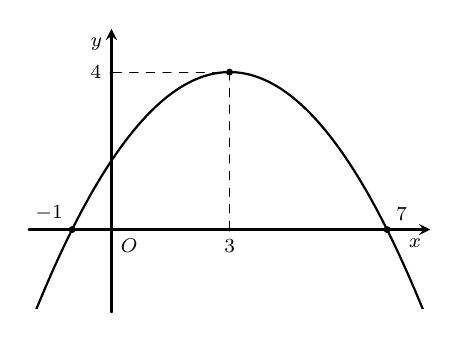
\begin{tikzpicture}[scale=0.5,line join=round,font=\footnotesize,line cap=round,>=stealth,thick]
				\tikzset{every  node/.style={scale=0.9}}
				\draw[->] (-2.1,0)--(8.1,0) node[below left] {$x$}; 
				 \draw[->] (0,-2.1)--(0,5.1) node[below left] {$y$};
				\draw (0,0) node  [below right] {$O$};
				\foreach \x/\nx in  {3/3}
				\draw[thin] (\x,1pt)--(\x,-1pt) node [below] {$\nx$}; 
				\foreach \y/\ny  in {4/4}
				\draw[thin] (1pt,\y)--(-1pt,\y) node  [left] {$\ny$};
				\draw[dashed,thin](3,0)--(3,4)--(0,4); 
				\begin{scope}
					 \clip (-2,-2) rectangle (8,5);
					 \draw[samples=200,domain=-2:8,smooth,variable=\x] plot (\x,{-0.25*(\x)^2+1.5*(\x)+1.75});
					\path (-1,0)  node[above left]{$-1$};
					\path (7,0) node[above  right]{$7$};
				\end{scope}
				\fill (3,4)  circle (2.5pt);
				\fill (-1,0)  circle (2.5pt);
				\fill (7,0)  circle (2.5pt);
			\end{tikzpicture}
		 }
	\loigiai{ 
		Dựa vào đồ thị ta thấy $(P)$ cắt  trục tung tại điểm có tung độ $y<4$.
	 }
\end{ex}

% nguồn: MaHoaNH_TracNghiem_Lop10
\begin{ex}%[0D3V2-4]%[ma:b877d548]
	Tìm  tất cả các giá trị của tham số $m$ để đồ thị hàm số $y=x^2+2 m x+m^2-3 m+1$ cắt trục hoành tại hai điểm phân biệt.
	 \choice
		{$m<\dfrac{1}{3}$} 
		 {$m=-1$}
		 {$m<0$}
		 {\True $m>\dfrac{1}{3}$}
	\loigiai{ 
		Đồ thị hàm số $y=x^2+2 m x+m^2-3 m+1$ cắt trục hoành  tại hai điểm phân biệt
		$\Leftrightarrow x^2+2 m  x+m^2-3 m+1=0$ có hai nghiệm phân biệt
		 $\Leftrightarrow \Delta^{\prime}=3 m-1>0 \Leftrightarrow m>\dfrac{1}{3}$.
	 }
\end{ex}

% nguồn: MaHoaNH_TracNghiem_Lop10
\begin{ex}%[0D3B2-4]%[ma:9bb4454d]
	Một  hộp đựng $ 12 $ bóng đèn trong đó có $ 4 $ bóng hỏng. Chọn ngẫu nhiên $ 3 $ bóng. Xác suất của biến cố $A\colon$ \lq\lq \textbf{Không} có bóng đèn nào hỏng\rq\rq~ là?
	 \choice
		{$\dfrac{28}{55}$} 
		 {$\dfrac{8}{55}$}
		{$\dfrac{7}{55}$} 
		 {\True $\dfrac{14}{55}$}
	 \loigiai{
		Số phần tử không gian mẫu là $  n(\Omega) =\mathrm{C}^3_{12}=220$.\\
		Số cách chọn ra ba bóng  không có bóng hỏng là $ n(A)=\mathrm{C}^3_{8}=56$.\\
		Xác suất cần tìm  là $ P(A)=\dfrac{14}{55} $.
	 }
\end{ex}

% nguồn: MaHoaNH_TracNghiem_Lop10
\begin{ex}%[0D3B2-4]%[ma:4abc7234]
	Một hộp chứa ba quả cầu trắng và hai quả cầu đen. Lấy ngẫu nhiên đồng thời hai quả cầu. Xác suất  để lấy được cả hai quả cầu trắng là
	\choice 
		{$\dfrac{4}{10}$} 
		 {\True $\dfrac{3}{10}$}
		{$\dfrac{2}{10}$} 
		{$\dfrac{5}{10}$} 
	\loigiai{ 
		Lấy ngẫu nhiên đồng thời hai quả cầu  từ hộp chứa $3$ quả cầu trắng và $2$ quả cầu đen, số kết quả có thể xảy ra là $n(\Omega)=\mathrm{C}_5^2=10$.\\
		Xét biến cố $A$: ``lấy được $2$ quả cầu trắng''.\\ 
		Số kết quả thuận lợi cho $A$ là $n(A)=\mathrm{C}_3^2=3$, do đó $\mathrm{P}(A)=\dfrac{n(A)}{n(\Omega)}=\dfrac{3}{10}$. 
	} 
\end{ex}

% nguồn: MaHoaNH_TracNghiem_Lop10
\begin{ex}%[0D3B2-4]%[ma:89fd4578]
	Một hộp có $5$ bi  đen, $4$ bi trắng. Chọn ngẫu nhiên $2$ bi. Xác suất $2$ bi được chọn có đủ hai màu là
	\choice 
		{\True $\dfrac{5}{9}$} 
		 {$\dfrac{2}{9}$}
		 {$\dfrac{5}{214}$}
		{$\dfrac{1}{18}$} 
	\loigiai{ 
		Chọn ngẫu nhiên $2$ bi từ hộp có $5$ bi đen, $4$ bi trắng, có $n(\Omega)=\mathrm{C}_9^2=36$ kết  quả có thể xảy ra.\\
		Biến cố  $A\colon$ ``$2$ bi được chọn có đủ $2$ màu'' có $n(A)=5\cdot 4=20$.\\
		 Vậy xác suất của $A$ là $\mathrm{P}(A)=\dfrac{n(A)}{n(\Omega)}=\dfrac{20}{36}=\dfrac{5}{9}$.
	} 
\end{ex}

% nguồn: MaHoaNH_TracNghiem_Lop10
\begin{ex}%[0D3Y2-4]%[ma:245c3455]
	Từ một hộp chứa $5$ quả cầu trắng, $6$ quả cầu đỏ, $7$ quả cầu vàng, các quả cầu có kích thước và khối lượng giống nhau, lấy ngẫu nhiên đồng thời $3$ quả cầu. Xác suất lấy được $3$ quả cầu có  ba màu khác nhau là
	 \choice
		 {$\dfrac{35}{68}$}
		{\True $\dfrac{35}{136}$} 
		{$\dfrac{11}{24}$} 
		{$\dfrac{11}{36}$} 
	 \loigiai{
		 Ta có $n\left(\Omega\right)=\mathrm{C}_{18}^3$.\\
		Gọi $A$ là biến  cố \lq\lq lấy được $3$ quả cầu có ba màu khác nhau \rq\rq.\\
		Suy ra $n\left(A\right)=5\cdot  6\cdot 7$.\\
		Do đó  $\mathrm{P}(A)=\dfrac{n(A)}{n(\Omega)}=\dfrac{35}{136}$.
	} 
\end{ex}

% nguồn: MaHoaNH_TracNghiem_Lop10
\begin{ex}%[0D3B2-4]%[ma:24b67bb2]
	 Có $3$ viên bi đỏ và $7$ viên bi xanh, lấy ngẫu nhiên $4$ viên bi. Tính xác suất để lấy được $2$ viên bi đỏ và $2$ viên bi xanh.
	\choice 
		 {$\dfrac{7}{10}$}
		 {\True $\dfrac{3}{10}$}
		{$\dfrac{4}{35}$} 
		 {$\dfrac{17}{35}$}
	\loigiai{ 
		Ta  có $n(\Omega)=\mathrm{C}_{10}^4=210$.\\
		Biến cố $A$ \lq\lq  Lấy được $2$ viên bi đỏ và $2$ viên bi xanh\rq\rq.\\
		Suy ra, $n(A)=\mathrm{C}_7^2\cdot\mathrm{C}_3^2=63$.\\ 
		Vậy xác suất biến cố $A$ là  $\mathrm{P}(A)=\dfrac{n(A)}{n(\Omega)}=\dfrac{63}{210}=\dfrac{3}{10}$.
	 }
\end{ex}

% nguồn: MaHoaNH_TracNghiem_Lop10
\begin{ex}%[0D3B2-4]%[ma:fc42560b]
	Một lô hàng gồm $1000$ sản phẩm, trong đó có $50$ phế  phẩm. Lấy ngẫu nhiên từ lô hàng đó $1$ sản
	phẩm. Xác suất để lấy được sản phẩm tốt là? 
	\choice 
		 {$0{,}94$}
		 {$0{,}96$}
		 {\True $0{,}95$}
		 {$0{,}97$}
	 \loigiai{
		Ta có  $n(\Omega)=\mathrm{C}_{1000}^1=1000$.\\
		Biến  cố $A$ \lq\lq Lấy được sản phẩm tốt\rq\rq.\\
		Suy ra,  $n(A)=\mathrm{C}_{950}^1=950$.\\
		Vậy xác suất  biến cố $A$ là $\mathrm{P}(A)=\dfrac{n(A)}{n(\Omega)}=\dfrac{950}{1000}=0{,}95$.
	} 
\end{ex}

% nguồn: MaHoaNH_TracNghiem_Lop10
\begin{ex}%[0D3B2-4]%[ma:952cfce6]
	Một lô hàng $20$ sản phẩm trong đó có $4$ phế phẩm. Lấy tùy ý $6$ sản phẩm từ lô hàng đó. Tính xác suất để $6$ sản phẩm  đó có không quá một phế phẩm.
	\choice 
		{$\dfrac{91}{285}$} 
		{\True $\dfrac{637}{969}$} 
		 {$\dfrac{7}{9}$}
		{$\dfrac{91}{323}$} 
	 \loigiai{
		Không gian mẫu  $\Omega$: \lq\lq Lấy 6 sản phẩm trong 20 sản phẩm\rq\rq \,suy ra $n(\Omega)=\mathrm{C}_{20}^6$.\\
		Biến cố $A$: \lq\lq Lấy 6 sản phẩm có không quá một phẩm\rq\rq\, suy ra $n(A)=\mathrm{C}_{16}^5  \cdot \mathrm{C}_4^1+\mathrm{C}_{16}^6$.\\
		Vậy xác  suất để $6$ sản phẩm đó có không quá một phế phẩm là:
		$$ 
		\mathrm{P}(A)=\dfrac{n(A)}{n(\Omega)}=\dfrac{\mathrm{C}_{16}^5  \cdot \mathrm{C}_4^1+\mathrm{C}_{16}^6}{\mathrm{C}_{20}^6}=\dfrac{637}{969}.
		 $$
	 }
\end{ex}


%%%%%%%%%%%%%%%% ĐÚNG/SAI %%%%%%%%%%%%%%%%

% nguồn: MaHoaNH_DungSai_Lop10
\begin{ex}%[0D3H2-4]%[ma:da38b850]
	Cho  hàm số bậc hai có đồ thị như hình vẽ
	\begin{center}
		\begin{tikzpicture}[scale=0.5]
				\draw[->] (-2,0)--(6.5,0)  node [below]{$x$};
				\draw[->] (0,-4.5)--(0,4)  node[left]{$y$};
				\node  (0,0)[below left]{$O$};
				 \draw (1,-0.1)--(1,0.1);
				\draw  (5,-0.1)--(5,0.1);
				\draw[dashed] (3,0)--(3,-4)--(0,-4); 
				\draw (1,0)  node[below left] {$1$};
				 \draw (3,0) node[above] {$3$};
				\draw  (5,0) node[below right] {$5$};
				\draw (0,-4)  node[left]{$-4$};
				\clip (-2.88,-5.3) rectangle (6.1,3.44); 
				\draw [samples=50,rotate around={0.:(3.,-4.)},xshift=3.cm,yshift=-4.cm,domain=-4.0:4.0)] plot (\x,{(\x)^2/2/0.5}); 
			\end{tikzpicture}
	\end{center}
	Các khẳng định sau đây đúng hay sai? 
	 \choiceTF
		 {Đồ thị hàm số bậc hai có đỉnh là $(-4;3)$}
		{\True Hàm số nhận giá trị âm  với mọi $x \in (1;5)$}
		{\True Đường thẳng $y=m$ cắt  đồ thị hàm số đã cho khi và chỉ khi $m >-4$}
		{Đường thẳng  $x=n$ cắt đồ thị hàm số đã cho khi và chỉ khi $n>0$}
	\loigiai{ 
		\begin{itemchoice}
			\itemch Đồ thị hàm số bậc hai  có đỉnh là $(3;-4)$
			\itemch Hàm số nhận giá trị âm với mọi $x \in (1;5)$ vì  trên $(1;5)$ đồ thị nằm dưới trục hoành.
			\itemch Đường thẳng $y=m$ cắt đồ  thị hàm số đã cho khi và chỉ khi $m >-4$
			\itemch Đường thẳng $x=n$ luôn cắt đồ thị  hàm số bậc hai với mọi $n$.
		\end{itemchoice}
	 }
\end{ex}

% nguồn: MaHoaNH_DungSai_Lop10
\begin{ex}%[0D3V2-4]%[0D3H2-2]%[0D3H2-3]%[0D3N2-1]%[ma:86c063f4]
	Cho hàm số bậc hai $y=2x^2+x-3$ có đồ thị $(P)$. Xét tính đúng sai của  mỗi mệnh đề dưới đây.
	 \choiceTF
		{Điểm $A(0; 3)$ thuộc đồ thị $(P)$} 
		{\True Đồ thị $(P)$ có tọa độ đỉnh là $I\left(-\dfrac{1}{4};-\dfrac{25}{8}\right)$} 
		{\True Hàm  số nghịch biến trên khoảng $(-\infty;-2)$ và đồng biến trên khoảng $(3;+\infty)$}
		{Có 5 giá trị nguyên dương $m\in[-3; 10)$ để đường thẳng $(d)\colon y=-(m+1) x-m-2$ cắt đồ thị $(P)\colon y=2 x^2+x-3$ tại hai  điểm phân biệt nằm về cùng một phía đối với trục tung}
	\loigiai{ 
		\begin{itemchoice}
			\itemch \textbf{ Sai}. Vì $3  \ne 2\cdot 0^2+0-3=-3$.
			 \itemch \textbf{ Đúng}. Vì $\heva{&-\dfrac{b}{2a}=-\dfrac{1}{4}\\& f\left( -\dfrac{b}{2a}\right) =-\dfrac{25}{8}} \Rightarrow I\left(-\dfrac{1}{4};-\dfrac{25}{8}\right)$.
			\itemch \textbf{ Đúng}. Hàm số có hệ số $a=2>0$ và $-\dfrac{b}{2a}=-\dfrac{1}{4}$ nên hàm  số nghịch biến trên khoảng $\left( -\infty; -\dfrac{1}{4}\right)$, đồng biến trên khoảng $\left( -\dfrac{1}{4};+\infty\right)$.\\
			Mà $(-\infty;-2)\subset\left( -\infty;  -\dfrac{1}{4}\right)$ và $(3;+\infty)\subset\left( -\dfrac{1}{4};+\infty\right)$.\\
			Do đó hàm số nghịch biến trên khoảng $(-\infty;-2)$ và đồng biến trên khoảng $(3;+\infty)$. 
			 \itemch \textbf{ Sai}. Xét phương trình
			$2x^2+x-3+(m+1) x+m+2=0 \Leftrightarrow 2 x^2+(m+2) x+m-1=0$. \tagEX{$*$}\noindent 
			Để phương trình $(*)$ có hai nghiệm phân biệt nằm về cùng một phía đối với trục  tung thì ta có điều kiện $\heva{&\Delta>0 \\ & P>0} \Leftrightarrow \heva{&m^2-4 m+12>0 \\ &\frac{m-1}{2}>0} \Leftrightarrow m>1$.\\
			Vậy có 8 giá trị nguyên dương  $m \in[-3; 10)$ để đường thẳng $(d)$ cắt đồ thị $(P)$ tại hai điểm phân biệt nằm về cùng một phía đối với trục tung.
		\end{itemchoice}
	} 
\end{ex}

% nguồn: MaHoaNH_DungSai_Lop10
\begin{ex}%[0D3V2-4]%[ma:3d555d2c]
	Cho hàm số $y= x^2-3x+1$ có đồ thị  $(P)$ và đường thẳng $d: y= x-m$.
	Các khẳng định sau đây đúng hay  sai?
	\choiceTF 
		 {Đường thẳng $d$ luôn song song với đường thẳng $\Delta : y = x$}
		{\True Khi $m=2$, đường thẳng $d$ cắt đồ thị $(P)$ tại hai điểm $(1;-1)$  và $(3;1)$}
		{Đường thẳng $d$ cắt đồ thị $(P)$ tại  hai điểm khi và chỉ khi $m<\dfrac{5}{2}$}
		{\True Đường thẳng $d$ cắt đồ thị $(P)$ tại hai điểm có hoành độ trái dấu khi và chỉ khi $m<-1$} 
	\loigiai{ 
		\begin{itemchoice}
			\itemch Khi  $m=0$ thì $d$ trùng với $\Delta$.
			\itemch Với $m=2$, $d: y=x-2$.  Phương trình hoành độ giao điểm
			\[ 
			 x^2-3x+1= x-2 \Leftrightarrow x^2-4x+3=0 \Leftrightarrow \hoac{&x=1\\&x=3.}
			 \]
			Suy ra đường thẳng $d$ cắt đồ thị $(P)$ tại hai điểm  $(1;-1)$ và $(3;1)$.
			\itemch Phương trình hoành độ  giao điểm
			\[ 
			x^2-3x+1=  x-m \Leftrightarrow x^2-4x+m+1 =0. \quad (1)
			\] 
			Đường thẳng $d$ cắt đồ thị $(P)$ tại hai điểm khi  và chỉ khi (1) có hai nghiệm phân biệt
			 \[
			\Leftrightarrow \Delta'=  4-m-1 >0 \Leftrightarrow m<3.
			 \]
			\itemch Đường thẳng $d$ cắt đồ thị  $(P)$ tại hai điểm có hoành độ trái dấu khi và chỉ khi phương trình
			 $x^2-4x+m+1 =0$ có hai nghiệm trái dấu $\Leftrightarrow m+1<0 \Leftrightarrow m<-1$.
		\end{itemchoice}
	} 
\end{ex}


%%%%%%%%%%%%%%%% TRẢ LỜI NGẮN %%%%%%%%%%%%%%%%

% nguồn: MaHoaNH_TraLoiNgan_Lop10
\begin{bt}%[0D3V2-4]%[ma:f4ea096c]
	Cho hàm số $y=2 x^2-5 x+2$ có đồ thị là parabol $(P)$. Tính tổng tất cả các hoành độ của giao điểm của  đồ thị với trục tung và trục hoành.
	 \shortans{2,5}
	 \loigiai{
		Từ  đề ta có: $a=2, b=-5, c=2$.\\
		Hoành độ của đỉnh $I$ là: $x_0=\dfrac{-b}{2 a}=\dfrac{-(-5)}{2.2}=\dfrac{5}{4}\Rightarrow y_0=2\left(\dfrac{5}{4}\right)^2-5 \cdot \dfrac{5}{4}+2=-\dfrac{9}{8}$ suy ra đỉnh  $I\left(\dfrac{5}{4};-\dfrac{9}{8}\right)$.\\
		Giao điểm của $(P)$ và trục $Oy$: Cho $x=0 \Rightarrow y=2$ nên $(P)$ cắt trục $O y$ tại điểm $A(0; 2)$. Giao điểm của $(P)$ và trục $Ox$: Xét phương trình $2 x^2-5 x+2=0 \Leftrightarrow\left[\begin{array}{l}x=2 \\ x=\dfrac{1}{2}
	\end{array}\right.$ nên $(P)$ cắt trục $O x$ tại hai điểm $B(2; 0)$ và $C\left(\dfrac{1}{2}; 0\right)$.\\
	Vậy  $0+2+\dfrac{1}{2}=2{,}5$.
 }
\end{bt}

% nguồn: MaHoaNH_TraLoiNgan_Lop10
\begin{bt}%[0D3V2-4]%[ma:a082731e]
	Cho parabol $(P): y=x^2-2x+m-1$. Biết tất cả các giá trị thực của $m$ để parabol cắt $Ox$  tại hai điểm phân biệt có hoành độ dương có dạng $a<m<b$. Tính $10^{ab}$.
	\shortans{100} 
	\loigiai{ 
		Phương trình hoành độ giao điểm  của $(P)$ và trục $O x$ là
		 $x^2-2 x+m-1=0$ $(1)$.\\
		Để parabol cắt $Ox$  tại hai điểm phân biệt có hoành độ dương khi và
		chỉ khi (1) có hai nghiệm phân biệt dương khi  và chỉ khi
		$$\heva{&\Delta^{\prime}=2-m>0\\&S=2>0\\&p=m-1>0}\Leftrightarrow\heva{&m<2\\&m>1}\Leftrightarrow  1<m<2.$$
		Vậy  $10^{ab} = 10^2 = 100$.
	 }
\end{bt}

% nguồn: MaHoaNH_TraLoiNgan_Lop10
\begin{bt}%[0D3V2-4]%[ma:55a4d877]
	Cho hàm số $f(x)=ax^2+bx+c$  $(a, b, c\in\mathbb{R})$ thỏa mãn $f(0)=1$ có bảng biến thiên như sau
	\begin{center}
		
\begin{tikzpicture}
				\tkzTabInit[nocadre=true,lgt=1.2,espcl=2.5,deltacl=0.5] 
					{$x$/0.7,$f  (x)$/2}
					 {$-\infty$,$1$,$+\infty$}
				\tkzTabVar 
					{+/$+\infty$,-/$-1$,+/$+\infty$ 
				 }
			\end{tikzpicture}
	\end{center}
	Có bao nhiêu giá trị nguyên của tham số $m$ để phương trình $f\left(f(x)+m\right)=1$  có đúng hai nghiệm phân biệt?
	 \shortans{1}
	\loigiai{ 
		Vì $f(x)$ là  đồ thị của một parabol có trục đối xứng là $x=1$ nên $f(0)=1$ thì $f(2)=1$. Suy ra
		\[f\left(f(x)+m\right)=1\Leftrightarrow \hoac{&f(x)+m=0\\&f(x)+m=2}\Leftrightarrow \hoac{&f(x)=-m\\&f(x)=2-m.} 
		 \]
		Để phương trình đã cho có đúng hai nghiệm phân biệt thì $\heva{&2-m >-1\\&-m <-1}\Leftrightarrow 1 < m  < 3$.\\
		Vậy có  $1$ giá trị nguyên của $m$ để phương trình đã cho có đúng hai nghiệm phân biệt.
	 }
\end{bt}


%%%%%%%%%%%%%%%% TỰ LUẬN %%%%%%%%%%%%%%%%

% nguồn: MaHoaNH_TuLuan_Lop10
\begin{bt}%[0D3V2-4]%[ma:5eb75048]
	Cho hàm số $y=-x^2+6x-5$ có đồ  thị là Parabol $(P)$. Tìm tât cả các giá trị của $m$ để đường thẳng $d:y=4x-m$ cắt đồ thị $(P)$ tại hai điểm phân biệt?
	\loigiai{ 
		Xét phương trình hoành độ giao  điểm của đường thẳng $d$ và đồ thị $(P)$ là
		$$ 
		-x^2+6 x-5=4  x-m \Leftrightarrow x^2-2 x+5=m .
		 $$
		Xét vế trái  $y=f(x)=x^2-2 x+5$, có $a>0$ suy ra $y=f\left(-\dfrac{b}{2 a}\right)=f(1)=4$ là giá trị nhỏ nhất. \\
		Vậy đường thẳng $d\colon y=4 x-m$ cắt đồ thị $(P)$ tại $2$ điểm phân biệt  khi $m>4$.
	 }
\end{bt}

% nguồn: MaHoaNH_TuLuan_Lop10
\begin{bt}%[0D3B2-4]%[ma:6f9f07b9]
	 (1.0 điểm)
	Một hộp đựng $ 7 $ bi xanh  và $ 6 $ bi đỏ. Chọn ngẫu nhiên $ 5 $ viên bi. Tính xác suất để $ 5 $ bi được chọn có đủ hai màu và số bi xanh nhiều hơn số bi đỏ.
	 \loigiai{
		Số  phần tử của không gian mẫu là $ n(\Omega) =\mathrm{C}^5_{13}= 1287$.\\
		Gọi $ A $ là biến cố~ \lq\lq $ 5 $ bi được chọn có đủ hai màu và số bi  xanh nhiều hơn số bi đỏ\rq\rq.\\
		Để chọn $ 5 $ bi được chọn có đủ hai màu và số bi xanh nhiều  hơn số bi đỏ ta có các trường hợp sau
		\begin{itemize}
			\item  [\bf TH1:] $ 3 $ xanh và $ 2 $ đỏ có $ \mathrm{C}^3_7 \cdot\mathrm{C}^2_6 =525$.
			\item [\bf TH2:]  $ 4 $ xanh và $ 1 $ đỏ có $ \mathrm{C}^4_7 \cdot\mathrm{C}^1_6 =210$.
		\end{itemize}
		Suy ra $ n\left(A\right)=735  $.\\
		 Xác suất cần tìm là $ P(A)= \dfrac{245}{429}$.
	 }
\end{bt}

% nguồn: MaHoaNH_TuLuan_Lop10
\begin{bt}%[0D3B2-4]%[ma:79c02afe]
	Giải  các phương trình sau
	\begin{enumerate}
		\item $\sqrt{x^2  + 3x - 3}=2x - 3$.
		\item $\sqrt{3x^2 - 2x + 3}=\sqrt{x^2  + 3x + 1}$.
	\end{enumerate}
	 \loigiai{
		\begin{enumerate}
			 \allowdisplaybreaks{
			\item \begin{eqnarray*}
			& &\sqrt{x^2 + 3x - 3}=2x -  3 \\
			 &\Leftrightarrow &\heva{& 2x-3\geq0 \\ & x^2+3x-3=(2x-3)^2}\\
			&\Leftrightarrow&\heva{& 2x\geq 3 \\ & x^2+3x-3=4x^2-12x+9}\\ 
			 &\Leftrightarrow &\heva{& x\geq\dfrac{3}{2} \\ & 3x^2-15x+12=0}\\
			&\Leftrightarrow&\heva{& x\geq\dfrac{3}{2} \\ & \hoac{& x=1  \mbox{ (loại)} \\ & x=4 \mbox{ (nhận)}.}}
		\end{eqnarray*}
		Vậy $x=4$. 
		\item \begin{eqnarray*}
		& &\sqrt{3x^2 - 2x + 3}=\sqrt{x^2 + 3x +  1}\\
		&\Leftrightarrow &\heva{&  x^2 + 3x + 1\geq0 \\ & 3x^2-2x+3=x^2 + 3x + 1}\\
		&\Leftrightarrow&\heva{& \hoac{& x\geq\dfrac{-3+\sqrt{5}}{2} \\ & x\leq\dfrac{-3-\sqrt{5}}{2}} \\  & 2x^2-5x+2=0}\\
		&\Leftrightarrow&\heva{& \hoac{& x\geq\dfrac{-3+\sqrt{5}}{2} \\ & x\leq\dfrac{-3-\sqrt{5}}{2}} \\  & \hoac{& x=2 \\ & x=\dfrac{1}{2}} \mbox{ (nhận)}.}
	\end{eqnarray*}}
	Vậy $x=2$,  $x=\dfrac{1}{2}$.
	\end{enumerate}
} 
\end{bt}
